\documentclass[tikz, border=3mm]{standalone}
\usepackage{amsmath,amssymb}
\usetikzlibrary{arrows.meta}

\begin{document}
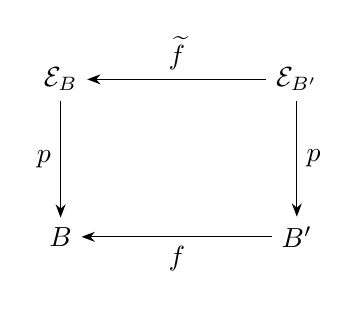
\begin{tikzpicture}[>=Stealth, node distance=3cm, auto]

% Nodes in total category (top row)
\node (EB)  at (0,2)  {$\mathcal{E}_B$};
\node (EBp) at (3,2)  {$\mathcal{E}_{B'}$};

% Nodes in base category (bottom row)
\node (B)   at (0,0)  {$B$};
\node (Bp)  at (3,0)  {$B'$};

% Arrows in the base
\draw[->] (Bp) to node[below]{$f$} (B);

% Vertical projection arrows
\draw[->] (EB)  to node[left] {$p$} (B);
\draw[->] (EBp) to node[right]{$p$} (Bp);

% Cartesian lifting (above f)
\draw[->] (EBp) to node[above]{$\widetilde{f}$} (EB);

\end{tikzpicture}
\end{document}
